\documentclass[10pt]{IEEEtran}
\pdfoutput=1

\usepackage{graphicx}
\usepackage{hyperref}
\usepackage[utf8]{inputenc}
\usepackage{listings}
\usepackage[table]{xcolor}
\usepackage{pdfpages}
\usepackage{float}
\usepackage[ruled,vlined]{algorithm2e}
\usepackage{caption}
\hypersetup{colorlinks=true,citecolor=[rgb]{0,0.4,0}}

\definecolor{green}{RGB}{39, 174, 96}

\title{Improving Trustpilot's rating system with data mining and machine learning}
\author{s094095 Steffen Karlsson \& S093475 Rune Thor Mårtensson}

\begin{document}
\maketitle

\begin{abstract}
The aim of this project is to improve the rating system of Trustpilot.dk, by utilizing data mining and machine learning. The way the improvement is supposed to work, is that a machine will be able to read reviews, get an understanding of what the customer is trying to convey about the company, and use the information to make a differentiated rating.
\end{abstract}

\section{Introduction}
When reading reviews at Trustpilot, you often see reviews which are very one-sided, only talking about how good a store is at handling delivery, how good their prices are or how good their pre-sales support is. The problem with Trustpilot's rating system is, that it is merely the average of all ratings for the company. As users do not touch on all subjects the system is inherently flawed, as a user who only touches one subject is rated the same as a user who touches all.

An example would be a customer writing a review, which only has information about how quick the company is to deliver a product. It is reasonable to presume, that the rating does not tell anything, about how good the company is at handling RMAs (Return Merchandise Authorization). 

By reading reviews and classifying the rating as something that is only related to delivery time, it is possible to make a differentiated rating, which this project achieves by using topic classification and sentiment analysis.

\section{Methods}
As the purpose of this project is to improve the rating system of a website, it makes sense to extend its functionality. This is achieved by using a \texttt{Greasemonkey}\cite{GreaseMonkey} script and an accompanying website which the script can acquire data from using \href{http://en.wikipedia.org/wiki/Ajax_(programming)}{\texttt{Ajax}}.
The system requires a web server, for this we use \href{http://httpd.apache.org/}{\texttt{Apache HTTP Server}}, as it is relatively easy to setup when using Linux. As the system needs to store data such as the differentiated ratings, a database is necessary, for which we use \href{http://www.mysql.com/}{\texttt{MySQL}}.

As the project is part of the course \href{http://www.kurser.dtu.dk/02819.aspx?menulanguage=en-GB}{02819 Data Mining using Python}, the project is coded in Python and uses language specific libraries.

\subsection{Data acquisition}
The system acquires data, by scraping Trustpilot's website, for which a framework was created, that extends the functionality of Pythons built-in \href{http://docs.python.org/2/library/htmlparser.html}{\texttt{HTMLParser}}. By using this framework, it is possible to define a parser using a simple syntax - that defines what elements from a HTML page that should be acquired - which improves maintainability, while keeping the performance advantages of using an event driven parser such as HTMLParser. As an event driven parser only iterates over the data once, it provide a performance advantage over other parsers such as \href{http://www.crummy.com/software/BeautifulSoup/}{\texttt{Beautiful Soup}}, which - depending on usage - can iterate over the same data more than once.

\subsection{Database}
To provide an interface to the database, the ORM (Object Relational Mapper) \href{http://peewee.readthedocs.org/en/latest/}{\texttt{peewee}} is used. Peewee provides an easy to use interface between Python and a SQL database, in addition to this it provides protection against the commonly known vulnerability \href{https://www.owasp.org/index.php/Top_10_2013-A1-Injection}{\texttt{SQL injection}}.

\begin{algorithm}[h!]
	\KwData{review}
 	\KwResult{differentiated scores for the review}
	\For{sentences in review}{
		total sentence count += 1\\
		score = calculate sentiment score\\
		topics = classify sentence\\
		general score += score\\
		\For{topic in topics}{
			topic score += score\\
			topic sentence count += 1
		}
		title topics = classify title\\
		title score = calculate sentiment score\\
		\For{topic in topics}{
			\eIf{topic is general}{
				topic score /= total sentence count
   			}{
  				\eIf{topic is in title topics}{
					topic score = (0.7 * topic score + 0.3 * title score) / topic sentence count
   				}{
  					topic score = (0.7 * topic score) / topic sentence count
  				}
  			}
  			add topic and score to differentiated score 		
		}
	} 	
\caption{Calculate differentiated scores for a review \label{alg:differentiated}}
\end{algorithm}

\begin{figure*}[!ht]
	\vspace*{10mm}
	\hspace*{25mm}	
	\begin{tabular}{ | l | c | c | c | c | r | }
  		\hline
   		 & \textbf{RMA} & \textbf{Price} & \textbf{Delivery} & \textbf{General} & \textbf{Original\footnote{Originally in the range 1-10, it has been converted to range 1-100}} \\ \hline
  		\href{http://www.trustpilot.dk/review/www.av-connection.dk}{AV-Connection} & 64.72 & 80.37 & 80.42 & 77.09 & 99 \\ \hline
  		\href{http://www.trustpilot.dk/review/www.conradelektronik.dk}{Conrad Elektronik Danmark} & 52.01 & 69.51 & 69.12 & 65.26 & 68 \\ \hline
  		\href{http://www.trustpilot.dk/review/www.sony.dk}{Sony}  & 45.00 & 49.44 & 55.78 & 50.75 & 29 \\ \hline
	\end{tabular}
	\hspace*{30mm}	
	\caption{Computed and original scores for three companies. \label{fig:scores}}
\end{figure*}

\subsection{Data processing}
When processing the acquired data, the system has two major components; the first is the multi topic classifier, which helps identifying topics within a review, the second component does sentiment analysis, which provides a positive or negative score for a review based on affective norms from the danish version of the word list AFINN-111\cite{IMM2011-06010}. The multi topic classifier has the ability to train an infinite number of the implementation of \href{http://nltk.org/api/nltk.classify.html#module-nltk.classify.naivebayes}{\texttt{Naïve Bayes classifers}} from nltk, which the system uses to classify review text in different categories.
\\~
\\~
To calculate the differentiated scores for a company, which is the aim of the project, it is necessary to calculate differentiated scores for every review. To do this the multi topic classifier and sentiment analysis is used in an algorithm, which has been created and the pesudo code is available at Algorithm \ref{alg:differentiated}.

\subsection{Website}
In addition to these components, the system has a simple website, which processes Ajax requests from users and holds the Greasemonkey script, information about the project and a link to the structured documentation generated with \href{http://sphinx-doc.org/}{\texttt{Sphinx}}. The website uses the Python web framework Flask, which helps serve all content while protecting against the known attack vectors \href{https://www.owasp.org/index.php/Cross-site_Scripting_(XSS)}{\texttt{XSS}} and \href{https://www.owasp.org/index.php/Cross-Site_Request_Forgery_(CSRF)}{\texttt{CSRF}}. The website is created using \href{http://getbootstrap.com/}{\texttt{Bootstrap}} with a slightly modified template from \href{http://bootswatch.com/flatly/}{\texttt{bootswatch.com}}, which makes it easy to design a website.

\subsection{Miscellaneous}
To allow administrators to use the system, it has a number of administrative scripts. Which makes it possible to create jobs that scrape reviews for a company, scrape companies from a category and compute ratings based on the scraped reviews. Jobs are executed using \href{http://pubs.opengroup.org/onlinepubs/009696699/utilities/crontab.html}{\texttt{cron}} which is a time based job scheduler found in Linux and Unix.
\\~
\\~
To help administrative tasks for this system, it implements logging to linux/unix standard logging facility \href{http://tools.ietf.org/html/rfc5424}{\texttt{syslog}}. At the moment it only logs to a local file, but in theory the system could be configured to log to a remote syslog.

The system is hosted on a micro instance from Amazon EC2, which runs the Debian GNU/Linux distribution. The system is hosted off-site, because it necessary to keep the system running 24/7 while acquiring data and serving results to users.

\section{Results}
By using this system, it is possible to generate the following results for three companies, one from the top, one from the middle and one from the bottom, in this order in the table \ref{fig:scores}.
\newpage
The same scores are shown in figure \ref{fig:scores_gui}, which also displays how the scores are integrated on Trustpilot's website, in a way that unobtrusive and elegant.

\begin{figure}[h!]
	\centering
	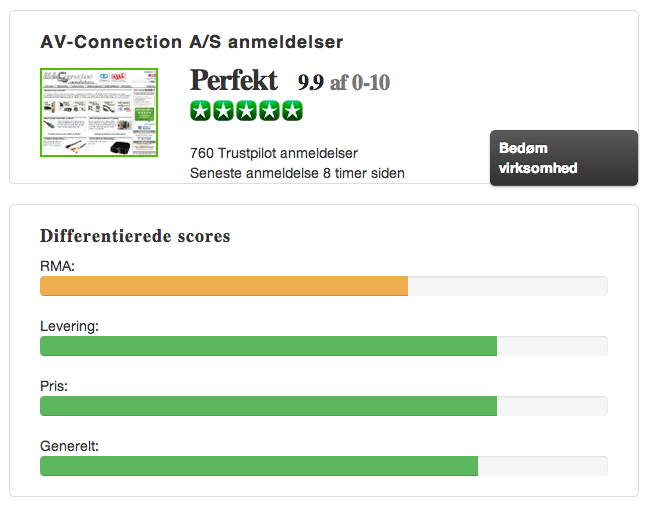
\includegraphics[scale=0.37]{scores.png}
	\caption{Integration of scores on Trustpilot. \label{fig:scores_gui}}
\end{figure}

\subsection{Code checking}
All code in the system has been checked with \href{http://www.pylint.org/}{\texttt{Pylint}}, which helps enforce the \href{http://www.python.org/dev/peps/pep-0008/}{\texttt{PEP 8}} standard. All relevant changes from Pylint have been implemented. However there is a few notable exceptions such as; R0904 "Too many public methods" which is not relevant when extending a class and R0903 "Too few public methods" which again is not relevant when methods are provided a super class, such as in the case of the data models from peewee, which is auto-generated from the database scheme. It should be noted that these messages should be ignored, and are merely a product of the standard configuration of Pylint, and could be ignored by using a custom configuration.

\subsection{Testing}


\subsection{Profiling}
During all parts of the design of this system, the focus has been on functionality as well as performance, as such there have not been any issues related to system performance.

However to showcase that the parser framework that was created is faster than Beautiful Soup, it has been profiled for memory consumption using the packages \href{https://pypi.python.org/pypi/memory\_profiler}{\texttt{memory\_profiler}} and \href{http://code.google.com/p/psutil/}{\texttt{psutil}}, and for execution time with Pythons built-in timeit functionality. The results are available in table \ref{fig:profiling}.

\begin{figure}[!h]
	\vspace*{2mm}
	\centering
	\begin{tabular}{ | l | c | c | }
  		\hline
   		 & \textbf{Beautiful Soup} & \textbf{HTML parser framework} \\ \hline
  		Min time & 0.954 & 0.614 \\ \hline
  		Max time & 0.971 & 0.636 \\ \hline
  		Avg time & 0.957 & 0.618 \\ \hline
  		Memory & 73.676 MiB & 13.887 MiB \\ \hline
	\end{tabular}
	\caption{Minimum, maximum and average time (on 1000 iterations) plus memory usage between the parser framework and Beautiful Soup. \label{fig:profiling}}
\end{figure}

The improvement relative to Beautiful Soup is that it is at least {\color{green} 34\%} faster and uses {\color{green} 430\%} less memory.

\section{Discussion}
As table \ref{fig:scores} shows, the system is able to generate scores, for the categories RMA, price, delivery and general. The first three are differentiated scores, which show how well a company is at handling this category, general is the overall feel of all reviews, which includes the previous three.

As expected all the companies in the table, shows a significantly lower score in the category RMA. Which to our experience is likely attributed to a fact, that users who have a good experience with RMA handling, will not report it, where as users who have a bad experience are more likely to report it.
\\~
\\~
It should be noted that sentiment analysis in general, is sensitive to irony and lack of affective norms. To mitigate this issue we have implemented words which amplify or negate the value of an affective norm. An example of a word that amplifies another is "very" as in "very good", and for negation "not" as in "not good".

In spite of it is always possible to improve the system, by increasing the amount of training data available for the multi topic classifier, which should increase the ratio of text that is classifiable.
\\~
\\~
The scores the system is able to generate, are not necessarily a mirror of the score that Trustpilot, has as overall score for the company. An example of this could be \href{http://www.trustpilot.dk/review/www.av-connection.dk}{AV-Connection}, where the score from Trustpilot is 9.9 out of 10, where it shows from the result that the store is significantly worse at handling RMA, compared to the other categories. 

\section{Conclusion}
We have accomplished in creating a system, which is able to compute differentiated scores for companies. 

The gamble that we took, by spending time on creating our own HTML parser framework paid off, it uses significantly less amount of memory as well as being at least 34\% faster.

\bibliographystyle{IEEEtran}
\bibliography{References}

\end{document}
